\section{Durchführung}
Zu Beginn werden sämtliche Bauteile deren Werte aufgezeichnet.
Für die Bestimmung des Dämpfungswiderstandes wird die Schaltung wie in Abbildung (\ref{fig:3}) dargestellt genutzt.
\begin{figure}[H]
\centering
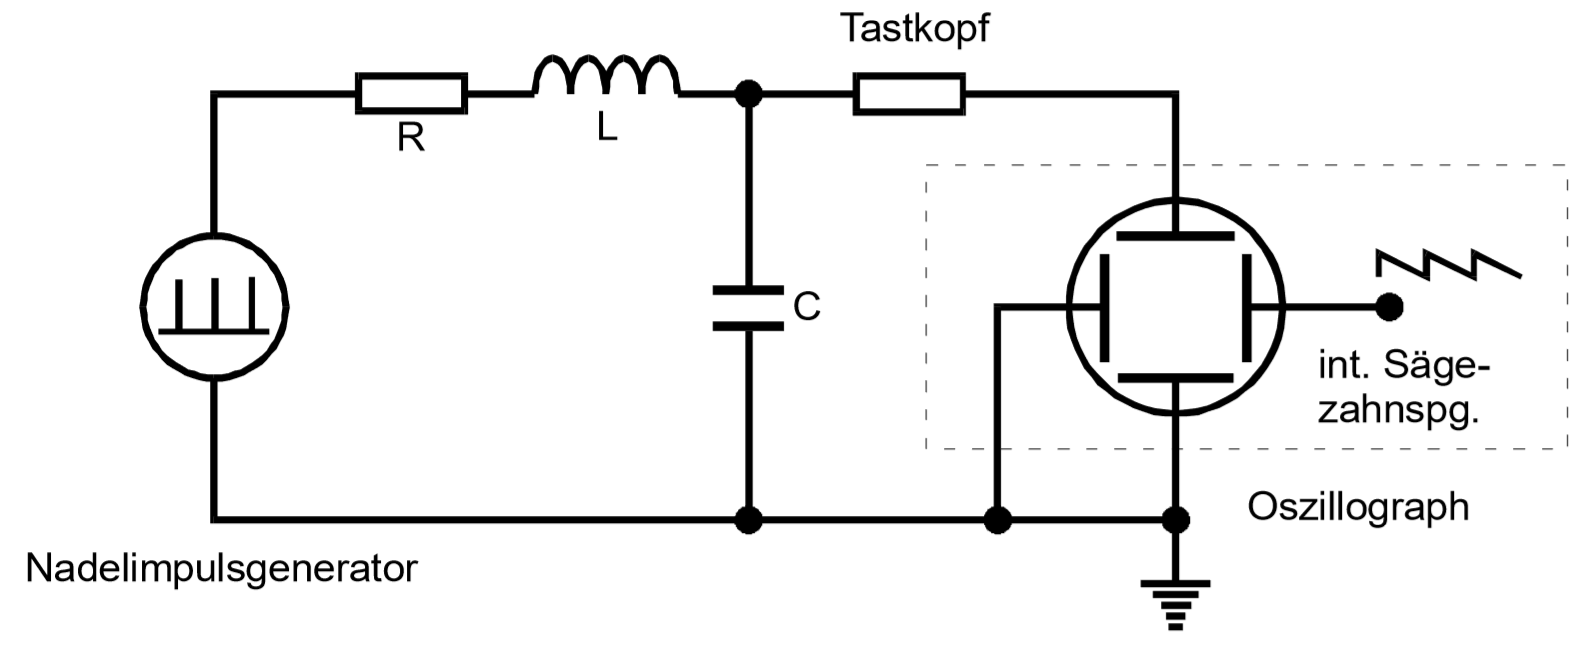
\includegraphics[width=\textwidth]{Schaltung1.png}
\caption{Schaltdarstellung zur Bestimmung des effetkiven Dämpfungswiderstandes[1].}
\label{fig:3}
\end{figure}
Mit Hilfe eines Oszilloskops wird die Kondensatorspannung gegen die Zeit dargestellt und ein Thermodruck ausgeführt.
Der Widerstand zur Messung des aperiodischen Grenzfalls wird ebenfalls mit Hilfe eines Oszilloskops und einem Potentiometer bestimmt.
Für die Messung der Phasenverschiebung und der Frequenzabhängigkeit der Kondensatorspannung wird die Schaltung wie in Abbildung (\ref{fig:4}) benötigt.
\begin{figure}[H]
\centering
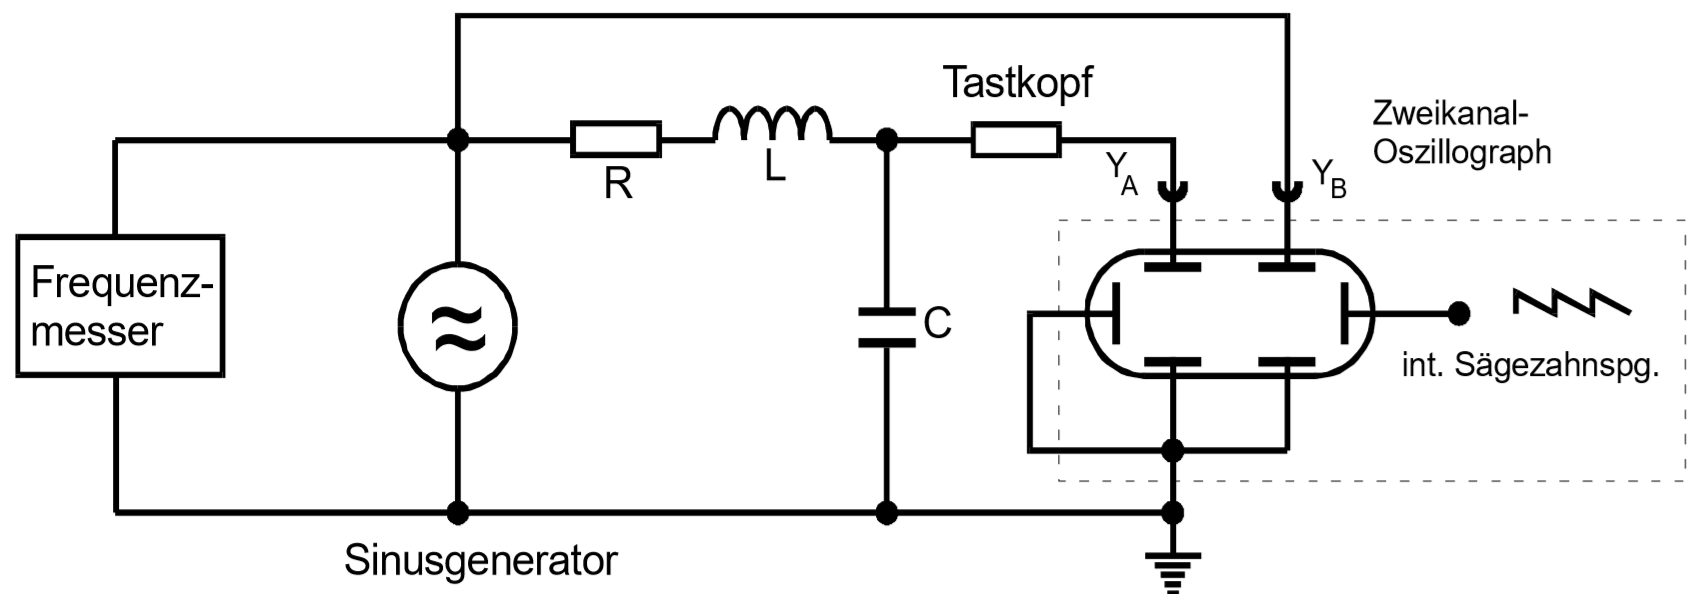
\includegraphics[width=\textwidth]{Schaltung2.png}
\caption{Schaltdarstellung zur Bestimmung der Phasenverschiebung[1].}
\label{fig:4}
\end{figure}
Zur Bestimmung der Phasenverschiebung wird wie in Abbildung (\ref{fig:5}) mit
 \begin{equation}
   \phi = \frac{a}{b} \cdot 360 \quad oder \quad \phi = \frac{a}{b} \cdot 2\pi
\end{equation}
   bestimmt.
\begin{figure}[H]
\centering
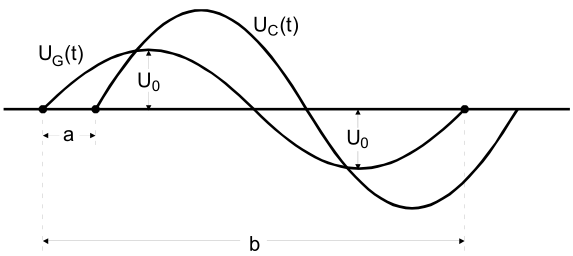
\includegraphics[width=\textwidth]{Phase.png}
\caption{Berechnung der Phasenverschiebung[2].}
\label{fig:5}
\end{figure}
